% *********************************************************************
% © 2016–2025 Jeremy Sylvestre
%
% Permission is granted to copy, distribute and/or modify this document
% under the terms of the GNU Free Documentation License, Version 1.3 or
% any later version published by the Free Software Foundation; with no
% Invariant Sections, no Front-Cover Texts, and no Back-Cover Texts. A
% copy of the license is included in the appendix entitled “GNU Free
% Documentation License” that appears in the output document of this
% PreTeXt source code. All trademarks™ are the registered® marks of
% their respective owners.
%
% *********************************************************************
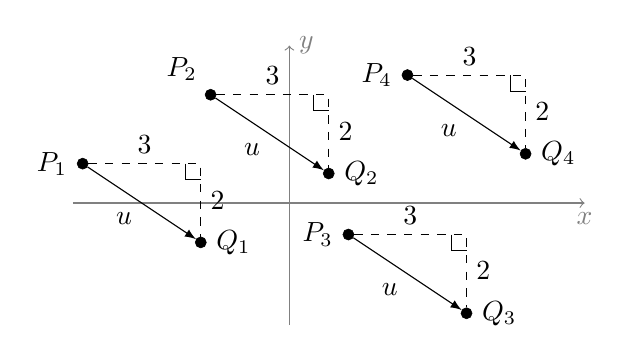
\begin{tikzpicture}[
	point/.style={circle,draw,very thin,fill,inner sep=0pt,minimum size=4pt},
	vector/.style={-latex},
	scale=0.5
]
	\draw[gray,->] (-5.5,0) to (7.5,0) node[below] {$x$};
	\draw[gray,->] (0,-3.1) -- (0,4) node[right] {$y$};
	\begin{scope}[xshift=-5.25cm,yshift=1cm]
		\node[point] at (0,0) (p) [label=left:$P_1$] {};
		\node[point] at (3,-2) (q) [label=right:$Q_1$] {};
		\draw[vector] (p) to node[below left] {$\uvec{u}$} (q);
		\draw[dashed] (p) to node[above] {$3$} (3,0) to node[right] {$2$} (q);
		\draw[very thin] (2.6,0) to (2.6,-0.4) to (3,-0.4);
	\end{scope}
	\begin{scope}[xshift=-2cm,yshift=2.75cm]
		\node[point] at (0,0) (p) [label=above left:$P_2$] {};
		\node[point] at (3,-2) (q) [label=right:$Q_2$] {};
		\draw[vector] (p) to node[below left] {$\uvec{u}$} (q);
		\draw[dashed] (p) to node[above] {$3$} (3,0) to node[right] {$2$} (q);
		\draw[very thin] (2.6,0) to (2.6,-0.4) to (3,-0.4);
	\end{scope}
	\begin{scope}[xshift=1.5cm,yshift=-0.8cm]
		\node[point] at (0,0) (p) [label=left:$P_3$] {};
		\node[point] at (3,-2) (q) [label=right:$Q_3$] {};
		\draw[vector] (p) to node[below left] {$\uvec{u}$} (q);
		\draw[dashed] (p) to node[above] {$3$} (3,0) to node[right] {$2$} (q);
		\draw[very thin] (2.6,0) to (2.6,-0.4) to (3,-0.4);
	\end{scope}
	\begin{scope}[xshift=3cm,yshift=3.25cm]
		\node[point] at (0,0) (p) [label=left:$P_4$] {};
		\node[point] at (3,-2) (q) [label=right:$Q_4$] {};
		\draw[vector] (p) to node[below left] {$\uvec{u}$} (q);
		\draw[dashed] (p) to node[above] {$3$} (3,0) to node[right] {$2$} (q);
		\draw[very thin] (2.6,0) to (2.6,-0.4) to (3,-0.4);
	\end{scope}
\end{tikzpicture}
